% Options for packages loaded elsewhere
\PassOptionsToPackage{unicode}{hyperref}
\PassOptionsToPackage{hyphens}{url}
%
\documentclass[
]{book}
\usepackage{lmodern}
\usepackage{amssymb,amsmath}
\usepackage{ifxetex,ifluatex}
\ifnum 0\ifxetex 1\fi\ifluatex 1\fi=0 % if pdftex
  \usepackage[T1]{fontenc}
  \usepackage[utf8]{inputenc}
  \usepackage{textcomp} % provide euro and other symbols
\else % if luatex or xetex
  \usepackage{unicode-math}
  \defaultfontfeatures{Scale=MatchLowercase}
  \defaultfontfeatures[\rmfamily]{Ligatures=TeX,Scale=1}
\fi
% Use upquote if available, for straight quotes in verbatim environments
\IfFileExists{upquote.sty}{\usepackage{upquote}}{}
\IfFileExists{microtype.sty}{% use microtype if available
  \usepackage[]{microtype}
  \UseMicrotypeSet[protrusion]{basicmath} % disable protrusion for tt fonts
}{}
\makeatletter
\@ifundefined{KOMAClassName}{% if non-KOMA class
  \IfFileExists{parskip.sty}{%
    \usepackage{parskip}
  }{% else
    \setlength{\parindent}{0pt}
    \setlength{\parskip}{6pt plus 2pt minus 1pt}}
}{% if KOMA class
  \KOMAoptions{parskip=half}}
\makeatother
\usepackage{xcolor}
\IfFileExists{xurl.sty}{\usepackage{xurl}}{} % add URL line breaks if available
\IfFileExists{bookmark.sty}{\usepackage{bookmark}}{\usepackage{hyperref}}
\hypersetup{
  pdftitle={DBG0061 - Portfólio},
  pdfauthor={João Vitor Ferreira Cavalcante},
  hidelinks,
  pdfcreator={LaTeX via pandoc}}
\urlstyle{same} % disable monospaced font for URLs
\usepackage{longtable,booktabs}
% Correct order of tables after \paragraph or \subparagraph
\usepackage{etoolbox}
\makeatletter
\patchcmd\longtable{\par}{\if@noskipsec\mbox{}\fi\par}{}{}
\makeatother
% Allow footnotes in longtable head/foot
\IfFileExists{footnotehyper.sty}{\usepackage{footnotehyper}}{\usepackage{footnote}}
\makesavenoteenv{longtable}
\usepackage{graphicx,grffile}
\makeatletter
\def\maxwidth{\ifdim\Gin@nat@width>\linewidth\linewidth\else\Gin@nat@width\fi}
\def\maxheight{\ifdim\Gin@nat@height>\textheight\textheight\else\Gin@nat@height\fi}
\makeatother
% Scale images if necessary, so that they will not overflow the page
% margins by default, and it is still possible to overwrite the defaults
% using explicit options in \includegraphics[width, height, ...]{}
\setkeys{Gin}{width=\maxwidth,height=\maxheight,keepaspectratio}
% Set default figure placement to htbp
\makeatletter
\def\fps@figure{htbp}
\makeatother
\setlength{\emergencystretch}{3em} % prevent overfull lines
\providecommand{\tightlist}{%
  \setlength{\itemsep}{0pt}\setlength{\parskip}{0pt}}
\setcounter{secnumdepth}{5}
\usepackage[utf8]{inputenc}
\usepackage[portuguese]{babel}
\usepackage{booktabs}
\usepackage{amsthm}
\makeatletter
\def\thm@space@setup{%
  \thm@preskip=8pt plus 2pt minus 4pt
  \thm@postskip=\thm@preskip
}
\makeatother
\usepackage[]{natbib}
\bibliographystyle{apalike}

\title{DBG0061 - Portfólio}
\author{João Vitor Ferreira Cavalcante}
\date{2020-06-19}

\begin{document}
\maketitle

{
\setcounter{tocdepth}{1}
\tableofcontents
}
\hypertarget{prefuxe1cio}{%
\chapter{Prefácio}\label{prefuxe1cio}}

Esse é o meu portfólio para a disciplina DBG0061 - RNAs Não Codantes, cursada no semestre suplementar 2020.5.

Aqui estarão contidas respostas para os exercícios de cada dia, dúvidas e reflexões sobre os seminários.

\hypertarget{aula1}{%
\chapter{mRNA, tRNA e rRNA}\label{aula1}}

\hypertarget{identifique-as-funuxe7uxf5es-de-cada-um}{%
\section{Identifique as funções de cada um}\label{identifique-as-funuxe7uxf5es-de-cada-um}}

\begin{itemize}
\item
  O mRNA é o responsável por carregar a informação codante do genoma, gerado no processo de transcrição,
  ele é o passo inicial para a produção de proteínas.
\item
  O tRNA é aquele que irá interpretar a informação contida no mRNA processado, se ligando aos seus códons e trazendo consigo o respectivo aminoácido.
\item
  O rRNA, por fim, será aquele responsável pela consolidação final da informação proteica, ao trafegar pelo mRNA, indica quais tRNAs devem se ligar e une os seus respectivos aminoácidos para a formação da proteína.
\end{itemize}

\hypertarget{regioes}{%
\section{Nomeie as regiões de um RNA mensageiro}\label{regioes}}

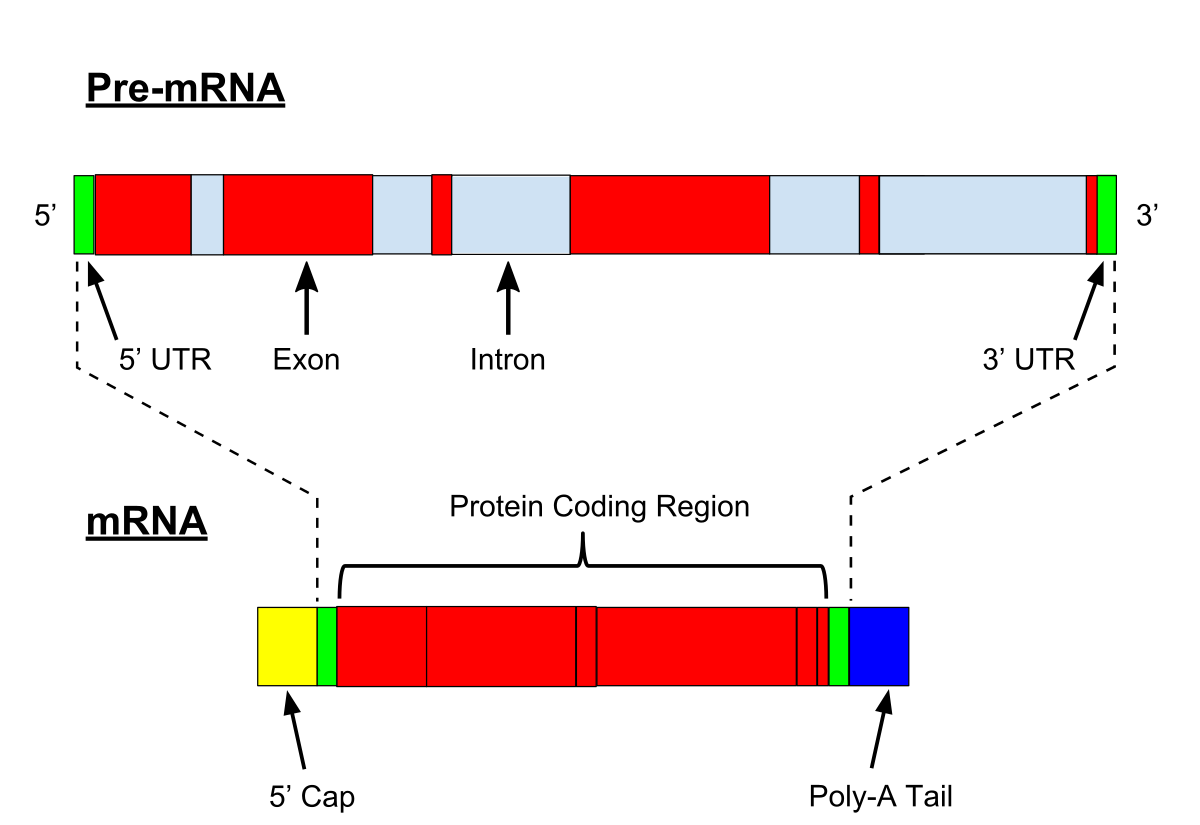
\includegraphics{./pics/estruturamrna.png}

Inicialmente, o mRNA possui 3 principais componentes: Os íntrons, que não codificam a informação proteica final, os éxons, a porção codante, e as UTRs em cada ponta, que são, também, regiões não traduzidas. Após o processamento, observa-se a adição de um ``capacete'' na extremidade 5' e uma sequência poli-A na extremidade 3', ambas estruturas que auxiliam na proteção do mRNA de exonucleases.

\hypertarget{gerauxe7uxe3o-e-modificauxe7uxf5es-puxf3s-transcricionais}{%
\section{Geração e modificações pós-transcricionais}\label{gerauxe7uxe3o-e-modificauxe7uxf5es-puxf3s-transcricionais}}

\hypertarget{mrna}{%
\subsection{mRNA}\label{mrna}}

A \textbf{transcrição}, em eucariotos, ocorre por meio da RNA Polimerase II, que junto a um ou mais fatores de transcrição, se liga
ao promotor, formando a bolha de transcrição, posteriormente, à medida que as ligações de hidrogênio vão sendo quebradas pela forquilha, vai se formando a fita, com a adição de nucleotídeos de RNA complementares. Ao fim deste processo teremos o pre-mRNA, que passará pelo processamento mencionado em \ref{regioes}

\hypertarget{trna}{%
\subsection{tRNA}\label{trna}}

Seus genes, localizados no nucléolo, são transcritos pela RNA Polimerase III. Em seguida ocorre o processamento do pre-tRNA formado, iniciando com a remoção de certas sequências, tanto na ponta 3' quanto na 5'. Vale destacar que inicialmente alguns tRNAs possuem íntrons, que em procariotos se auto-removem, mas em eucariotos e arqueas são removidos por endonucleases, que reconhecem sua região BHB. Por fim, há a adição de CCA na sua extremidade 3', posteriormente a isso o tRNA ainda pode passar por diversos processamentos, a depender do aminoácido ao qual se relaciona.

E, ultimamente, é claro, há a reação de aminoacilação quando o tRNA for executar sua função na célula.

\hypertarget{rrna}{%
\subsection{rRNA}\label{rrna}}

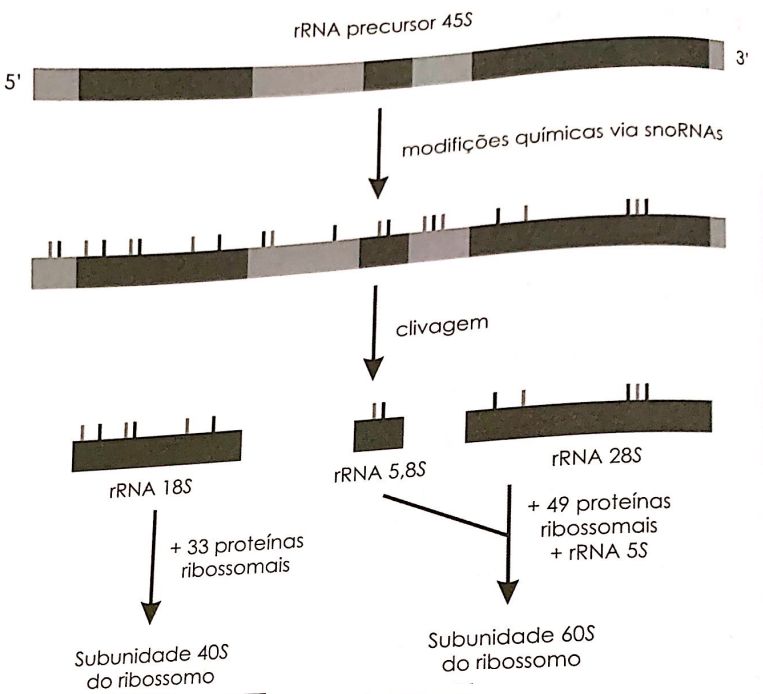
\includegraphics{./pics/rRNA synthesis.png}

Em eucariotos, ocorre no nucléolo, com a síntese do 45S pela RNA Polimerase I, este possuinte de regiões interespaçadas transcritas que assemelham íntrons, e no núcleo, com a síntese do 5S pela RNA Polimerase III. O 45S, após passar por modificações realizadas por snoRNAs, como metilação e pseudouridilação, tem seus espaçadores clivados. Os fragmentos resultantes se unem a proteínas ribossomais, formando as duas subunidades conhecidas, a 40S e a 60S.

\hypertarget{ediuxe7uxe3o-de-rna}{%
\section{Edição de RNA}\label{ediuxe7uxe3o-de-rna}}

É o processo no qual ocorrem modificações no RNA que não refletem mutações na sequência genômica original. Essas modificações podem ser inserções, deleções e substituições. Algumas modificações de nota são:

\begin{itemize}
\item
  Edição do gene da ApoB - uma troca de C para U - reflete nas isoformas observadas da proteína no organismo, a ApoB-100 (hepática) e a ApoB-48 (intestinal), essa última que possui seu tamanho reduzido pois a troca gera um códon de parada.
\item
  Conversão de A para Inosina pela \textbf{ADAR} em miRNAs, que pode impedir o processamento por DROSHA e DICER.
\end{itemize}

  \bibliography{book.bib}

\end{document}
